\documentclass[a4paper,11pt]{article}

\usepackage[latin1]{inputenc}
\usepackage[T1]{fontenc}
\usepackage{bbm} %math chars
\usepackage{amsmath}
\usepackage{indentfirst}
\usepackage{fullpage} %minimizes the default margins
\usepackage{url}
\usepackage{graphicx}
\usepackage[center,footnotesize]{caption} %options des legendes des graphes
\usepackage[section]{placeins} %place les figures d'une section avant le debut de la suivante
\usepackage{subfig} %a) b) c)

\title{Exercises - Week 6}
\date{}
\author{Genomics and bioinformatics}

\begin{document}
\maketitle

\section{Phylogenetic trees}

\begin{enumerate}
\item Start with the highest BLAST score (984) and link the two corresponding proteins (mm\_per2 and dr\_per2). Then continue with the next highest scores until the tree is completed. Because of the query and reference lengths, you noticed that BLAST scores are not symmetric, but following this rule there is a unique solution tree. 

\begin{center}
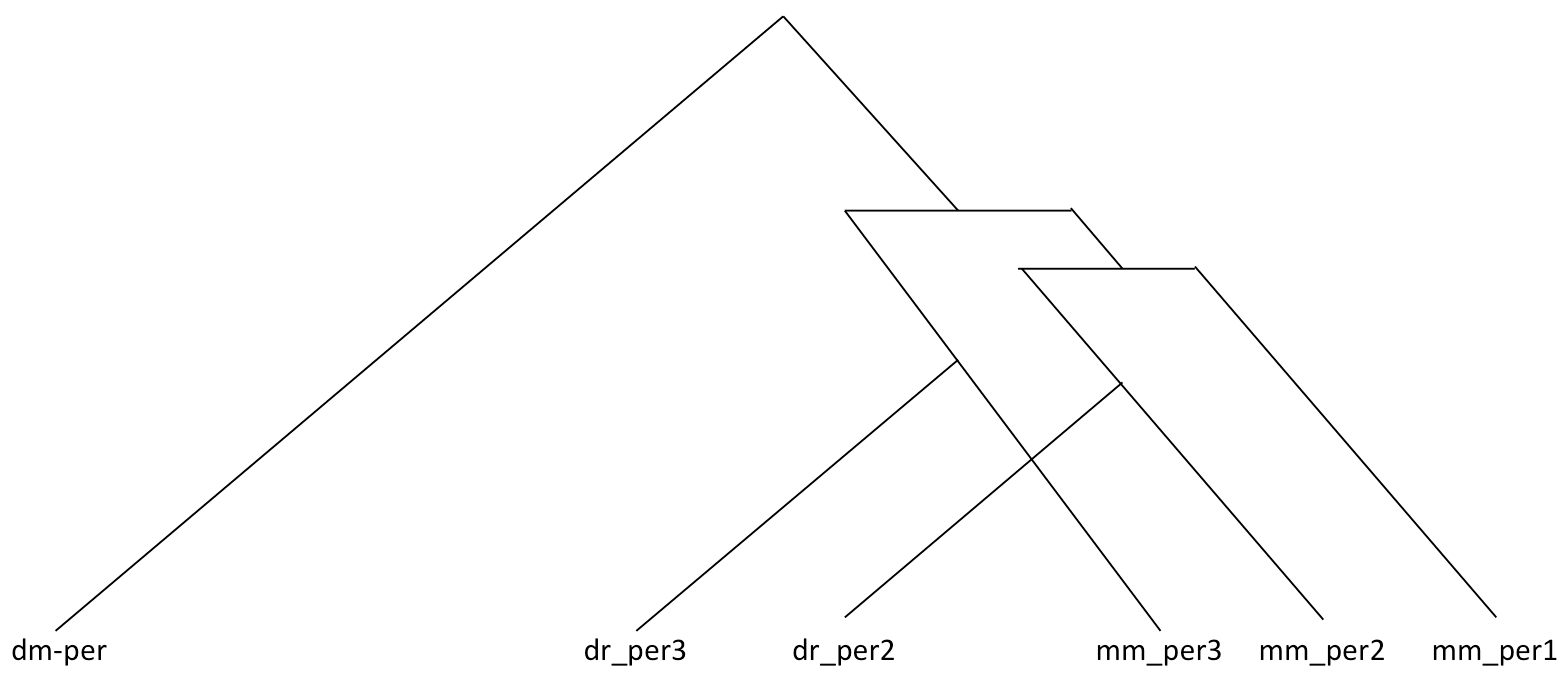
\includegraphics[width=0.8\textwidth]{tree.png}\\
\vspace{0.5cm}
{\bf The gene tree}
\end{center}

On this graph duplications events are represented with horizontal lines.
One can differentiate speciation and duplication events by the fact that we see the same species (but another version of the gene) on two branches separated by a duplication (as for {\bf mm\_per1} and {\bf mm\_per2}). When there is a speciation event, species are all different on both parts after the event (as for {\bf dm\_per} and {\bf dr\_per3}).

\item 
\begin{itemize}
	\item Orthologous pairs correspond to reciprocal best hits \emph{between two different species}. Here is the way to find them:\\
Choose one line of the table, say {\bf dm\_per}. Compare with the fish: on our line, the best score between {\bf dr\_per2} 
and {\bf dr\_per3} is 125 for {\bf dr\_per3}.
Then take the {\bf dm\_per} column, and verify that the same gene has the best score among dr genes. 
In this case, {\bf dr\_per3} is best with 123, compared to 114. So {\bf dm\_per} and {\bf dr\_per3} are reciprocal best hits, thus they are orthologs by definition.

Here is the list of orthologs:\\
{\bf dm\_per} and {\bf dr\_per3} \\
{\bf dm\_per} and {\bf mm\_per1} \\
{\bf dr\_per2} and {\bf mm\_per2} \\
{\bf dr\_per3} and {\bf mm\_per3} \\

\emph{Note:} in particular with this definition there are genes issued from speciation events that are not formally orthologs.
Closest pairs (such as {\bf dr\_per2} and {\bf mm\_per2}) are always orthologs.

	\item Non-reciprocal best hits are considered as paralogous pairs. In the same species: {\bf mm\_per1} and {\bf mm\_per2}.

	\item A paralogous pair in different species: {\bf mm\_per1} and {\bf dr\_per2}.
\end{itemize}
\end{enumerate}

\section{Another HMM}

\subsection{The Viterbi algorithm} 

Characters $T_1$, $T_2$ and $T_3$ are respectively A, T and C.
Choose a cell in the table: its position defines $n$ and $s$. Then replace emission and transition probabilities in the Viterbi formula.

Be careful here that if there is 0.8 probability of emitting one of A-T, there is 0.4 probability of emitting A and 0.4 for T; similarly for G-C.

\begin{center}
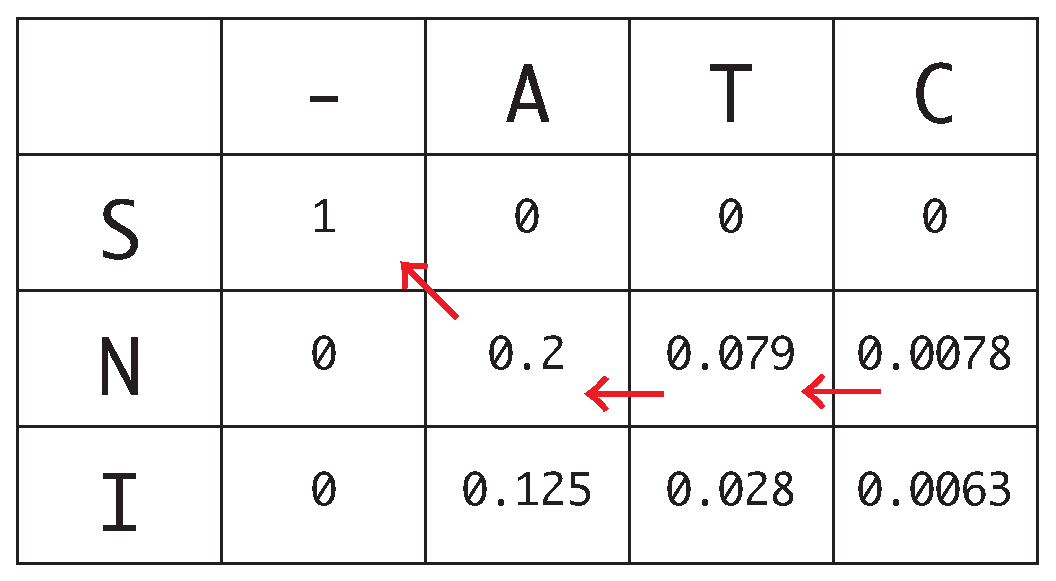
\includegraphics[width=0.5\textwidth]{fig3.eps}\\
\vspace{0.5cm}
\end{center}
The most probable hidden sequence associated to $ATC$ is $NNN$.

%\subsection{Using R}

%Comments...

\end{document}











